\chapter{Experimental setup}

\intro{The measurements within this thesis are based on proton-proton~(\gls{pp}) collision data recorded with the CMS detector in 2012, 2015, and 2016 at center-of-mass energies of 8 and 13~TeV. In this chapter the experimental setup is described. First, the \gls{lhc}, its preacceleator chain and the experiments at the \gls{lhc} are briefly described. Then, the CMS detector and its components are detailed. The chapter is concluded with a brief overview of the data acquisition system.}

%##############################################
\section{Large Hadron Collider}
%##############################################

The \glsreset{lhc}\gls{lhc} is a 26.7~km long accelerator and storage ring for protons and heavy ions at the \glsreset{cern}\gls{cern} located in the vicinity of Geneva, Switzerland. It was constructed between 1998\range2008 in the existing tunnel of the former \glsreset{lep}\gls{lep} which lies 45\range170~m below the surface of Switzerland and France. The \gls{lhc} ring features two beam pipes which can be separately filled with up to 2'808 countercycling bunches of protons with a bunch-to-bunch spacing of 25~ns per pipe. The two beams can be focused to cross each other at four \glspl{ip}. The design allows to accelerate protons with a momentum of 450~\GeV at injection to up to 7~\TeV yielding a center-of-mass energy of 14~\TeV in collisions.

To bend the beams 1'232 dipol cryostats are deployed hosting both beam pipes and two dipol magnets within a cold mass in a twin-bore design. The cold mass itself is placed in a vacuum vessel for thermal insulation. The magnet coils consist of \gls{nbti}  cables which are cooled down to 1.9~K using superfluid helium. At this temperature, the \gls{nbti} alloy is superconducting. This allows to produce the required dipol field strength ranging from 0.54~T at injection to up to 8.33~T at the maximum beam energy for sustaining a closed beam orbit. At maximum field a current of 11850~A is required. Such high magnetic fields cannot be achieved with normal conductors due to magnetic saturation. 

In addition to the dipol magnets about 3'800 single aperture and 1'000 twin aperture magnets are installed. Quadrupole magnets keep the beam particles focused around the nominal orbit. Further, non-linear corrections to the orbit are applied using sextu-, octu-, and decapoles. Special quadrupole triplets at each side of the four \glspl{ip} focus the beams for collision. The envelop of the particle trajectories with respect to the nominal beam orbit is described by the beta function which can be approximated around the \glspl{ip} as 

\begin{equation}
\beta(x)\approx\beta^\star+\frac{x^2}{\beta^\star}.
\end{equation}

In design, the beams can be squeezed to $\beta^\star=0.55~\mathrm{m}$ at two high luminosity \glspl{ip}. The transverse beam size is given as $d_{x,y}=\sqrt{\epsilon_\mathrm{n}\cdot\beta^\star/\gamma}\approx17\upmu\mathrm{m}$ for $\gamma=E_\mathrm{p}/m_\mathrm{p}=7000$ where $\epsilon_\mathrm{n}$ denotes the normalized beam emittance. It is a measure of the phase space area occupied by the particles within the beam which is constant following Liouville's theorem. The emittance cannot be larger than $\epsilon_\mathrm{n}>3.75~\upmu\mathrm{m}\cdot\mathrm{rad}$ in order to not loose significant amounts of the beam in the \gls{lhc} arcs where $\beta(x)$ is the largest.

For acceleration and longitudinal focusing, a system of eight superconducting cavity per beam with a resonance frequency of $400.8~\mathrm{MHz}$ are installed. This matches the 35640~harmonic mode of the beam revolution frequency of $f_\mathrm{rev}=11'245~\mathrm{Hz}$. The cavity system yields an energy gain per turn of 485~keV which results in an acceleration time of about 20~min from injection to the maximum beam energy.

The expected luminosity at the \glspl{ip} can be calculated from the introduced machine and beam parameters as

\begin{equation}
L=\frac{N_\mathrm{p}^{2}\,n_\mathrm{b}\,f_\mathrm{rev}}{4\pi\,d^2_{x,y}}\cdot F,\qquad F=\frac{1}{\sqrt{1+\big(\theta\cdot d_{z}\big)^2\big/\big({2\,d_{x,y}}\big)^2}}
\end{equation}

where $N_\mathrm{p}$ denotes the number of protons per bunch and $n_\mathrm{b}$ the number of colliding bunches. The design proton population per bunch is $N_\mathrm{p}=1.15\cdot10^{11}$. The factor $F$ accounts for a reduction in luminosity due to the slightly tilted beams by a crossing angle $\theta$.

In 2016, the design luminosity of $10^{34}~\mathrm{cm}^{-2}\mathrm{s}^{-1}$ was surpassed through various new developments~\cite{Team:2229040}. In detail these were a decrease of the transverse emittance, a smaller longitudinal bunch size, a better focusing at the \glspl{ip} down to $\beta^\star=0.4~\mathrm{cm}$, and a smaller crossing angle compared to the design values which resulted in a peak luminosity of about $1.5\cdot 10^{34}~\mathrm{cm}^{-2}\mathrm{s}^{-1}$. An overview of the peak luminosities per day in \gls{pp} collisions recorded by the CMS experiment from 2010--2016 is shown in Fig.~\ref{fig:experiment-peaklumi}. In Run~1~(2010--2012) the \gls{lhc} produced pp collisions at center-of-mass energies of 7 and 8~TeV. After the first long shutdown~(\gls{ls1}), the center-of-mass energy was raised to 13~TeV in Run~2 which started in 2015.

\myfigure{\label{fig:experiment-peaklumi}Peak luminosity in proton-proton collision data per day recorded by the CMS experiment. The figure is taken from the public luminosity result web page of CMS~\cite{lumipublic}.}{
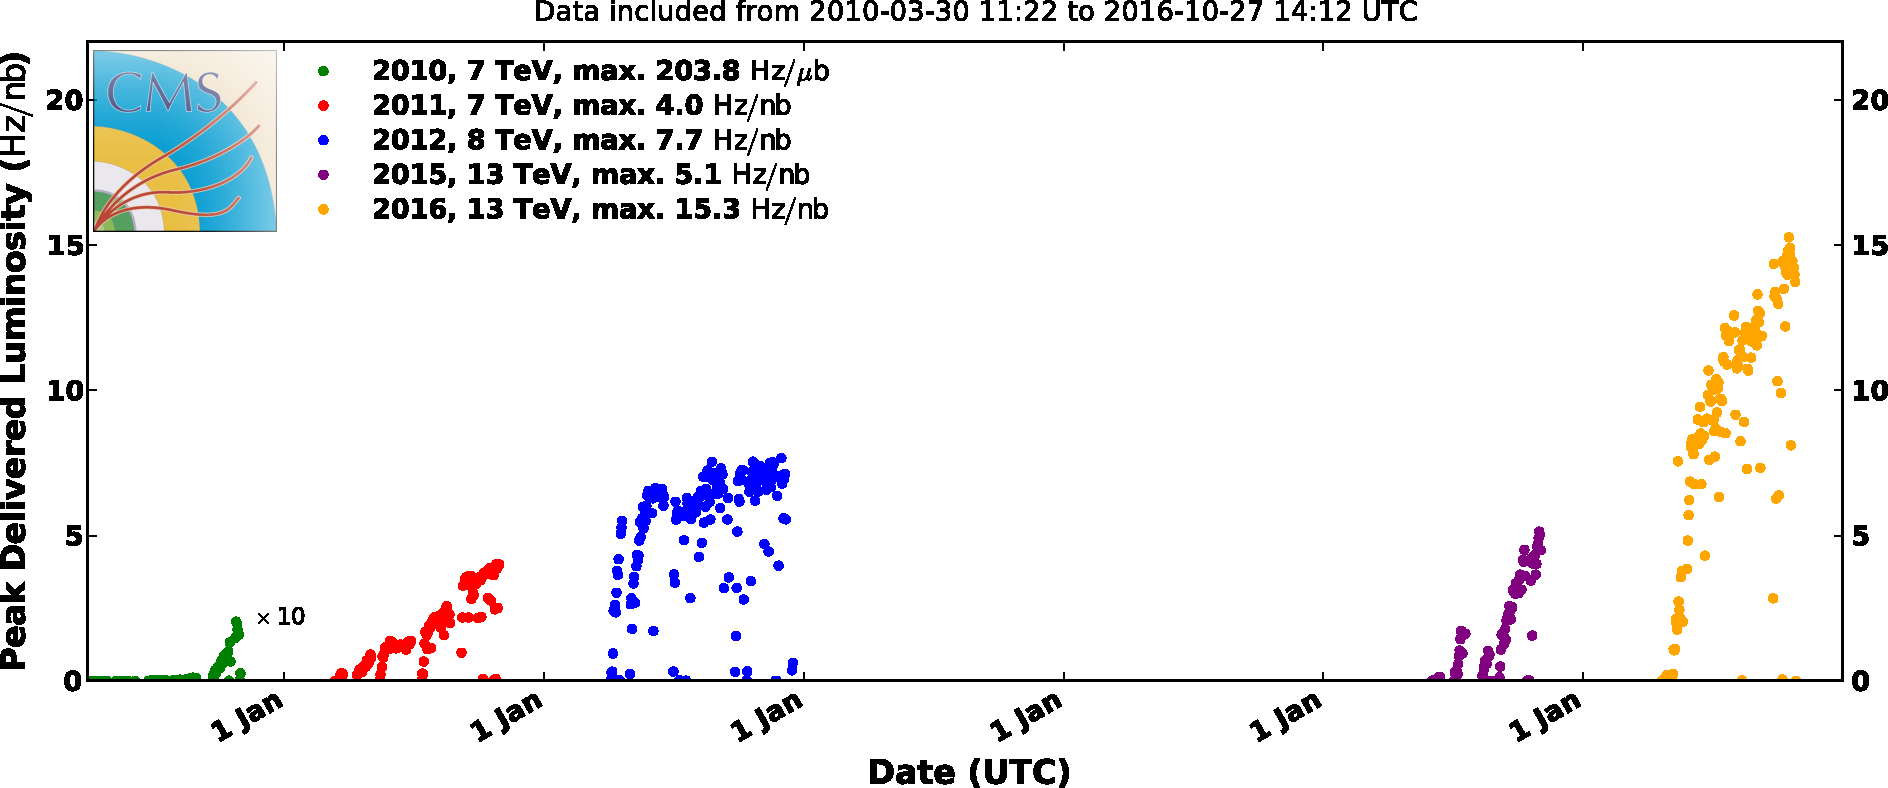
\includegraphics[width=0.95\textwidth]{figures/experiment/peak_lumi_pp.pdf}
}

During a bunch crossing multiple proton-proton interactions can occur which are referred to as \gls{pu}. Their number on average is proportional to the luminosity and the total inelastic \gls{pp} cross section. In 2012, an average number of 21 pileup interactions has been observed in 8~\TeV \gls{pp} collisions. This increased in 2016 due to the higher luminosity and cross section at 13~\TeV to ??? interaction per bunch crossing. \todo{no pu number found}


More information on the \gls{lhc} and its design parameters can be found in Ref.~\cite{Evans:2008zzb}.



%##############################################
\subsection{Accelerator complex}
%##############################################

An overview of the accelerator complex at \gls{cern} is given in Fig.~\ref{fig:experiment-accelerator-complex} which includes the systems for filling the \gls{lhc} with bunches of protons or lead ions.

\myfigure{\label{fig:experiment-accelerator-complex}The accelerator complex at \gls{cern}. The figure is taken from Ref.~\cite{Mobs:2225847}.}{
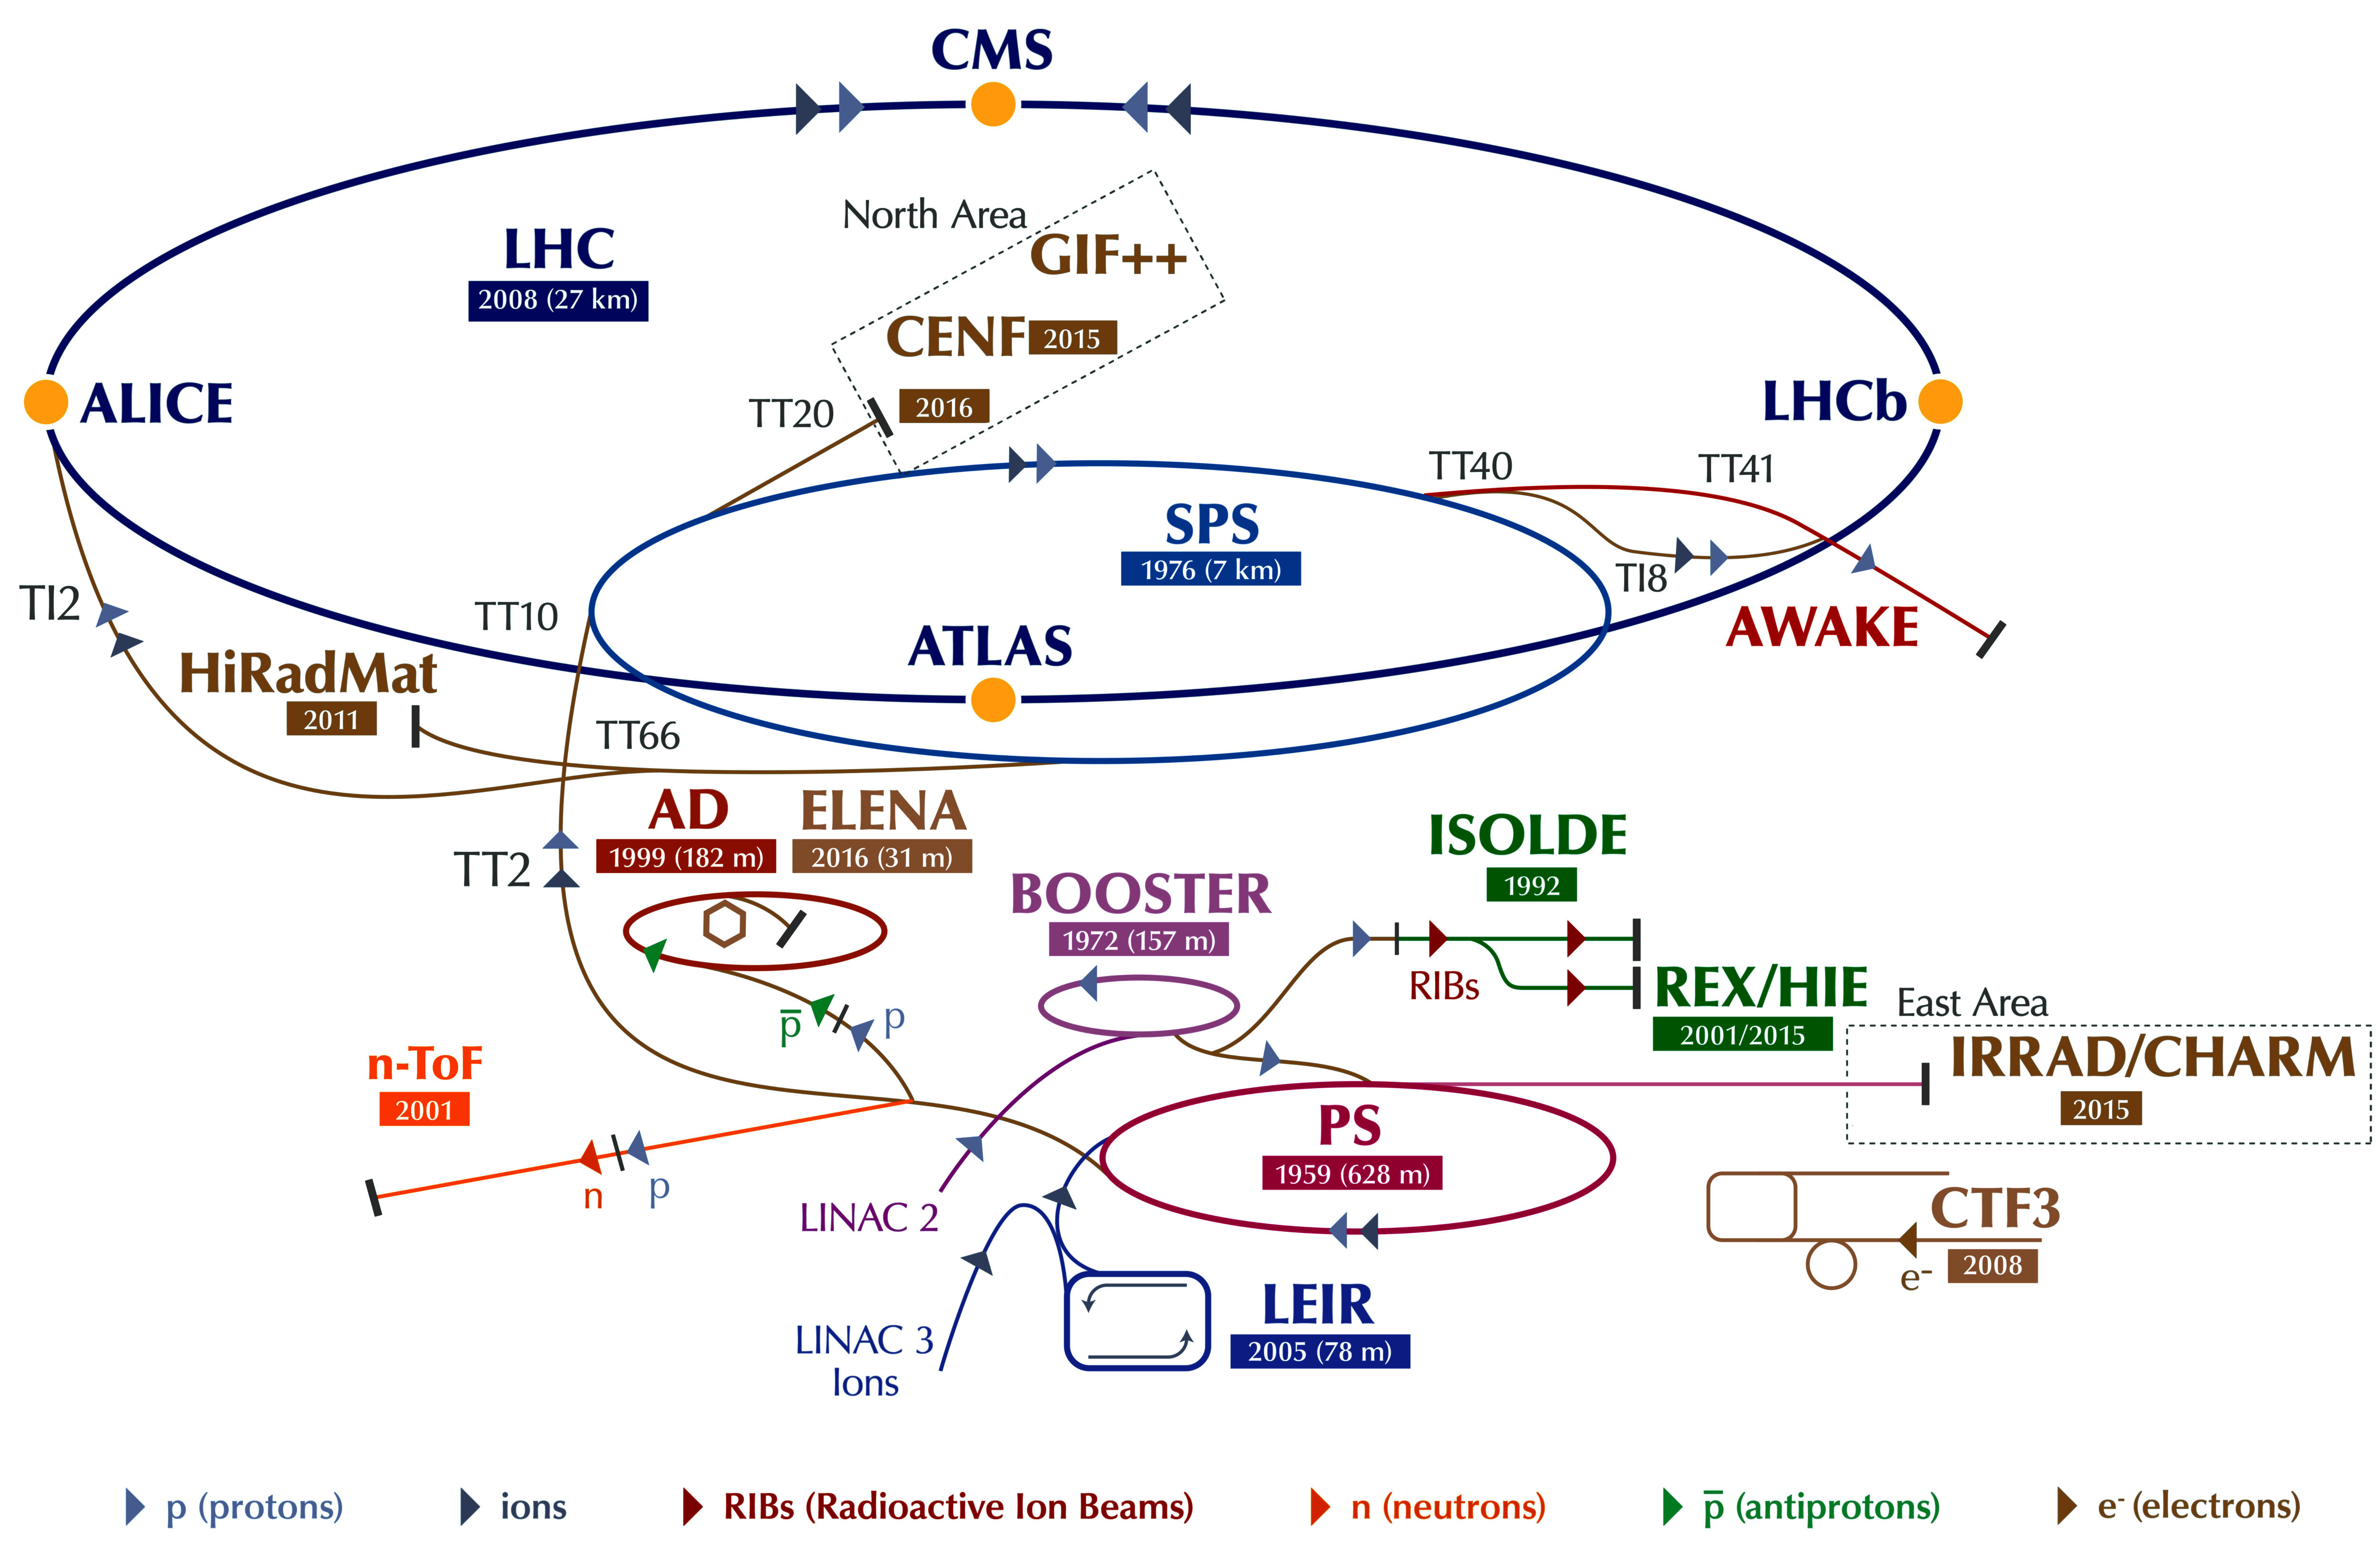
\includegraphics[width=0.99\textwidth]{figures/experiment/CERN_accelerator_complex.jpg}
}

The production sequence of proton bunches for the \gls{lhc} is as follows. In the linear accelerator ``Linac~2'', hydrogen atoms are stripped of their electron through an electric field. The remaining protons are accelerated to a momentum of 50~\MeV and injected into the \glsreset{psb}\gls{psb}. It consists of four vertically separated beam pipes which allow multi-turn injections to increase the bunch intensity which however also increases the transverse emittance~\cite{doi:10.1142/S0217751X13300196}. After accelerating the protons to 1.4~\GeV, the beams are injected into the \glsreset{ps}\gls{ps}. Here the required bunch spacing of 25~ns is formed. Until recently the standard procedure was to use only six bunches from two \gls{psb} cycles and split them first by three, accelerate them to 25~\GeV, and then split each again by two twice to produce in total 72~bunches with the required spacing~\cite{Benedikt:2001ar}. A new scheme called \gls{bcms} was introduced in 2016. It utilizes all eight bunches from two \gls{psb} cycles which are first narrowed and then combined to four followed by the same splitting and acceleration procedure as before which results in 48~bunches with higher intensity and lower transverse emittance~\cite{bcms}. Finally, the protons are injected and accelerated in the \glsreset{sps}\gls{sps} up to the \gls{lhc} injection energy of 450~GeV.

\todo{gap? beam life and filling time?}



%##############################################
\subsection{Overview of experiments}
%##############################################

Various particle detectors are installed at the \gls{lhc} to record the outcome of proton-proton or heavy ion collisions. Four major detectors are directly located at the \glspl{ip}. 

Two general purpose detectors are located at two high luminosity \glspl{ip}. These are the \gls{atlas}~\cite{Aad:2008zzm} and \gls{cms}~\cite{Chatrchyan:2008aa} experiments which have both a wide physics program ranging from precision measurements of the \glsunset{sm}\gls{sm} to the search for various kinds of new physics like extra dimensions, dark matter particles or \gls{susy}. Despite similar goals the technical realization of the two experiments is different. The \gls{atlas} detector is of cylindrical shape around the beam pipe with a length of 44~m and a diameter of 25~m. It consists of an inner detector, a liquid argon electromagnetic calorimeter, a hadronic calorimeter, and a muon spectrometer with full $2\uppi$ coverage in the azimuthal angle. %The inner detector is placed within a solenoid producing a magnetic field of 2~T for tracking of charged particles. A toroidal magnetic field with an average strength of 0.5~T allows to determine the momenta of muons in the outer spectrometer. 
A detailed description of the \gls{cms} detector is given in Sec.~\ref{sec:experiment-cms}.

The two other major detectors are the \gls{alice}~\cite{Aamodt:2008zz} and \gls{lhcb}~\cite{Alves:2008zz} experiments which are more specialized. Their luminosity is intentionally leveled down by displacing the beams slightly at their \glspl{ip}~\cite{Follin:1955354}. The lower luminosity is required to reduces the number of pileup interactions and to prevent damage to the detectors through radiation. The \gls{alice} experiment focuses on heavy ion collisions in which the properties of quark-gluon plasma can be studied. The goals of the \gls{lhcb} experiment are precision measurements of \gls{cp}-violation and searches for rare decays of B~hadrons amongst others.

Three additional smaller experiments, \gls{lhcf}~\cite{Adriani:2008zz}, \gls{totem}~\cite{Anelli:2008zza}, and \gls{moedal}~\cite{Pinfold:2009oia}, have been installed at the \gls{lhc} using certain fractions of the forward scattered particles from the \glspl{ip} of the \gls{atlas}, \gls{cms}, and \gls{lhcb} detectors respectively. 


%##############################################
\section{CMS experiment}
%##############################################
\label{sec:experiment-cms}

The \gls{cms} experiment is a multipurpose particle detector whose goal is to record pp and heavy ion collisions at the highest luminosities the \gls{lhc} can deliver. It consists of a superconducting solenoid and multiple subdetectors shown in Fig.~\ref{fig:experiment-cms} to track, reconstruct, and identify particles which traverse the detector each bunch crossing.

\myfigure{\label{fig:experiment-cms}Overview of the \gls{cms} subcomponents. The figure is taken from Ref.~\cite{Chatrchyan:2008aa}.}{
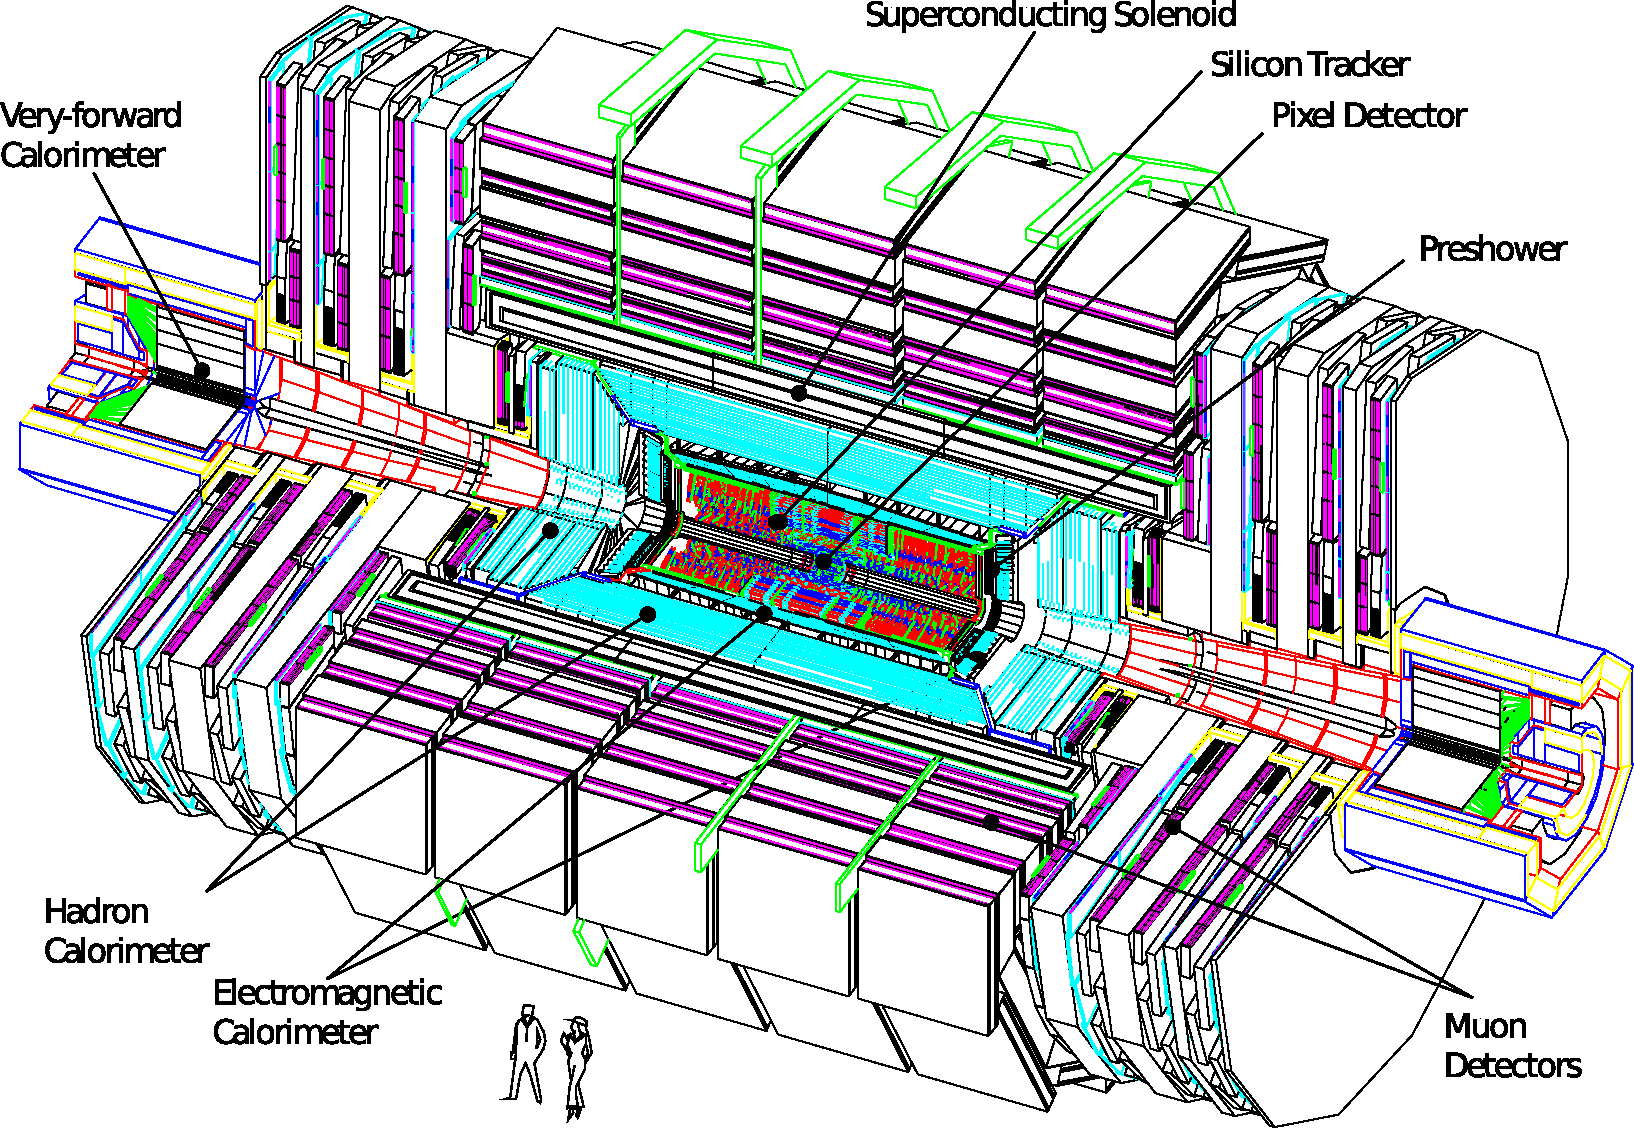
\includegraphics[width=0.99\textwidth]{figures/experiment/CMS_overview.pdf}
}

The detector is shaped cylindrically by layers in the barrel region and endcap disks in the forward regions around the beam pipe. It has an overall length of 21.6~m and a diameter of 14.6~m with a total weight of approximately 12'500~tons. A coordinate system has been established whose center is located at the nominal \gls{ip}. It is oriented such that the y-axis points upwards, the x-axis points inwards to the center of the \gls{lhc} ring, and the z-axis points along the beam pipe. The azimuthal angle $\phi$ is defined in the transverse plane, spanned by the x- and y-axes, which lies perpendicular to the beam pipe. In this plane, the radius is defined as $r=\sqrt{x^2+y^2}$ which measures the distance to the z-axis. For a particle originating from the center with an energy $E$ and momentum $p_\mathrm{z}$ along the z-axis one defines its rapidity as

\begin{equation}
y=\frac{1}{2}\ln\left(\frac{E+p_\mathrm{z}}{E-p_\mathrm{z}}\right). \label{eq:experiment-rapidity}
\end{equation}

The advantage of the rapidity over the usage of the angle $\theta$ measured from the z-axis is that differences of rapidities are invariant under Lorentz-boosts. Furthermore, in the case of a massless particle, the rapidity is equal to the pseudorapidity which is given as

\begin{equation}
\eta=\mathrm{artanh}\left(\frac{p_\mathrm{z}}{|\vec{p}|}\right)=-\ln\left[\tan\left(\frac{\theta}{2}\right)\right]. \label{eq:experiment-pseudorapidity}
\end{equation}

In the following, the components of \gls{cms} are briefly described and their purpose is motivated. More information can be found in Refs.~\cite{Chatrchyan:2008aa,Bayatian:922757}.


%##############################################
\subsection{Magnet}
%##############################################

The solenoid magnet is a crucial part of the \gls{cms} detector. It enables momentum measurements of charged particles by analyzing their curved trajectories with the inner tracker. Additionally, the curved trajectories of muons can be independently measured a second time in the outer return flux by the muon systems. The design of \gls{cms} was particularly motivated to achieve a good resolution of muon momenta and dimuon mass spectra which are a key ingredient when searching for new resonances like the at that time undiscovered Higgs boson decaying to four muons~\cite{Acquistapace:1997fm}.

The magnet consists of four layers of superconducting \gls{nbti} cables. It is placed in a cold mass within a vacuum tank which is cooled down to 4.6~K using liquid helium. In design it is capable of producing a homogeneous magnetic field of up to 4~T in its inner free bore with a length of 12.5~m and a diameter of 6~m. However, the magnet has been operated with a reduced current of 18164~A so far yielding a slight reduced field of 3.8~T until its aging is better understood~\cite{Chatrchyan:2009si}. 

To guide the return flux of the magnetic field, a large iron yoke has been installed. It consists of 12-sided barrel wheels in three layers with a length of 11~m and six endcap disks.

%##############################################
\subsection{Inner tracking system}
%##############################################

The inner tracking system is located closest to the beam pipe and has a total length of 5.8~m with a diameter of 2.5~m. It is used to find trajectories of charged particles which are bent by the magnetic field. Their momentum, charge, and point of origin can then be determined from the reconstructed track. 

At design luminosity, approximately 1'000 particles traverse the tracking system on average at each bunch crossing. This yields a hit rate density of about $1~\mathrm{MHz/mm^2}$ at the inner radius of 4~cm is which reduces to $3~\mathrm{kHz/mm^2}$ at the outer edge of the tracker. The sensor modules are based on doted silicon semiconductors which are operated in reverse mode to detect the traversing of charged particles through ionization. This technology allows for modules with a high granularity and a fast response time which are also able to operate in the such high radiation environments.

The system consists of various parts with different module types as shown in Fig~\ref{fig:experiment-tracker}. It covers a pseudorapidity range of $|\eta|<2.5$.

\myfigure{\label{fig:experiment-tracker}Overview of the \gls{cms} tracking system. The figure is taken from Ref.~\cite{Chatrchyan:2014fea}.}{
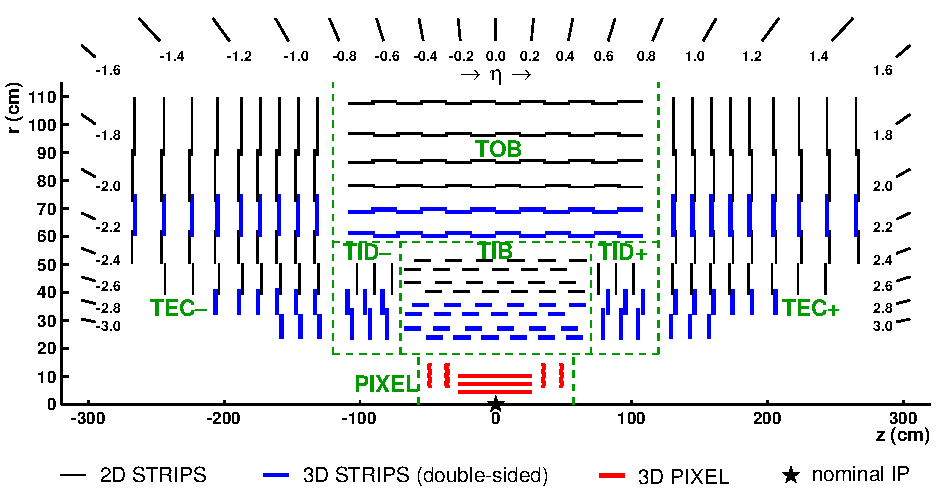
\includegraphics[width=0.99\textwidth]{figures/experiment/CMS_tracker.pdf}
}

Pixel modules are located next to the beam pipe where the particle flux is particularly high. They are installed in three barrel layers~(\gls{bpx}) at radii of 4.4, 7.3, and 10.3~cm, and in two endcap disks~(\gls{fpx}) per side. A pixel module has a cell size of $100\times150~\upmu\mathrm{m}^{2}$ which allows local 2D hit position measurements. Local positions are transformed into global 3D positions by accounting for the surface orientation of each module. The channel occupancy of the pixel subdetector which is defined as the fraction of active readout channels has been measured in data and ranges between 0.002\range0.02\% only~\cite{Chatrchyan:2014fea}. This facilitates the search for particles trajectories by generating seeds from precise hits on the pixel modules.

Silicon strip modules are installed in the other parts of the inner tracking system. The strip modules allow to measure a local 1D hit position perpendicular to the strip direction. A few layers and disks contain however double-sided strip modules as indicated in Fig.~\ref{fig:experiment-tracker}. These modules are tilted with an angle of 0.1~rad with respect to each other which allows to reconstruct matched 2D hits by combining 1D hits from both sides. The modules are organized in four inner barrel layers~(\gls{tib}) at radii of 20\range50~cm; six outer barrel layers~(\gls{tob}) at radii of 55\range116~cm; three inner endcap disks~(\gls{tid}); and nine outer endcap disks~(\gls{tec}). In the barrel the strip directions on each module are aligned along the z-axis with a strip-to-strip distance that varies between $80\range183~\upmu\mathrm{m}$. In the endcap disks, the modules are wedge-shaped with their strips running along the radial axis whose distance ranges between $100\range184~\upmu\mathrm{m}$. The modules are cooled down and operated below $-10^\circ\mathrm{C}$ to counteract the heat produced by the electronics and to improve their lifetime.

%##############################################
\subsection{Electromagnetic calorimeter}
%##############################################

The electromagnetic calorimeter~(\gls{ecal}) encloses the inner tracker and covers a pseudorapidity range of $|\eta|<3$. It consists of scintillating lead tungstate~($\mathrm{PbWO}_{4}$) crystals to detect electromagnetic showers emitted from charged or neutral particles (especially photons and electrons) in the crystals. In particular, the capability to detect a diphoton resonance from Higgs bosons which decayed to two photons has been one of its design goals.

Figure~\ref{fig:experiment-ecal} displays an overview of its layout. In total, 61'200 crystals with the shape of a truncated pyramid are installed in the barrel and 7'324 in each of the two endcaps. The barrel crystals have a length of 2.3~cm and a rectangular front cross section of $22\time22~\mathrm{mm}^{2}$. In the endcaps the crystals have a similar shape with a length of 2.2~cm and a front cross section of $28.62\times28.62~\mathrm{mm}^{2}$. The crystals are slightly tilted such that no particle originating from the nominal \gls{ip} can pass the \gls{ecal} through a crack within its acceptance.

\myfigure{\label{fig:experiment-ecal}Overview of the \gls{cms} electromagnetic calorimeter system. The figure is taken from Ref.~\cite{Bayatian:922757}.}{
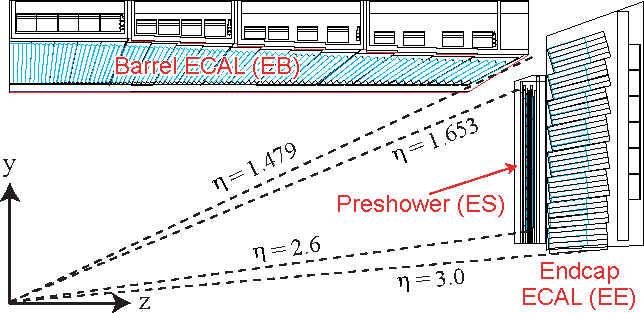
\includegraphics[width=0.75\textwidth]{figures/experiment/CMS_ecal.pdf}
}

The crystal material was chosen for its high density of $8.28~\mathrm{g}/\mathrm{cm}^{3}$, short radiation length of 0.89~cm, and radiation hardness. In addition, the spatial extend of an electromagnetic shower inside the crystals, the so-called Moli\`ere radius, amounts to only 2.2~cm which yields a good position resolution and shower separation. The crystals emit about 4.5 photoelectrons per \MeV with a wavelength of 420\range430~nm. About 80~\% of the light is emitted within 25~ns after an electromagnetic shower occurred. The photons are collected and their signal is amplified by \glspl{apd} in the barrel. In the endcaps \glspl{vpt} are deployed instead which are specifically designed to operated also in the axial magnetic field.

In front of the two \gls{ecal} endcaps, the preshower detector~(\gls{es}) is located which covers a pseudo rapidity range of $1.652<|\eta|<2.6$. The preshower allows to identify neutral pions and improves the identification and position of electrons and photons. It consists of two layers of lead radiators to initiate electromagnetic showers with a layer of silicon strip sensors after each radiator to measure the transverse profile of a shower.

%##############################################
\subsection{Hadron calorimeter}
%##############################################

The hadron calorimeter~(\gls{hcal}) is a sampling calorimeter and organized in four parts as shown in Fig.~\ref{fig:experiment-hcal}. It covers a pseudorapidity range of $|\eta|<5$ in total. Its function is to initiate and detect hadronic showers from particles such as protons, neutrons, kaons, and pions which allows to measure their position and energy. Furthermore, it helps to determine the net missing transverse energy of an event since the only remaining particles from a collision that are not stopped by the \gls{hcal} are neutrinos and muons where the latter are however identified in the muon systems as discussed later in Sec.~\ref{sec:experiment-muon-systems}.

\myfigure{\label{fig:experiment-hcal}Overview of the \gls{cms} hadronic calorimeter system. The figure is taken from Ref.~\cite{Chatrchyan:2008aa}.}{
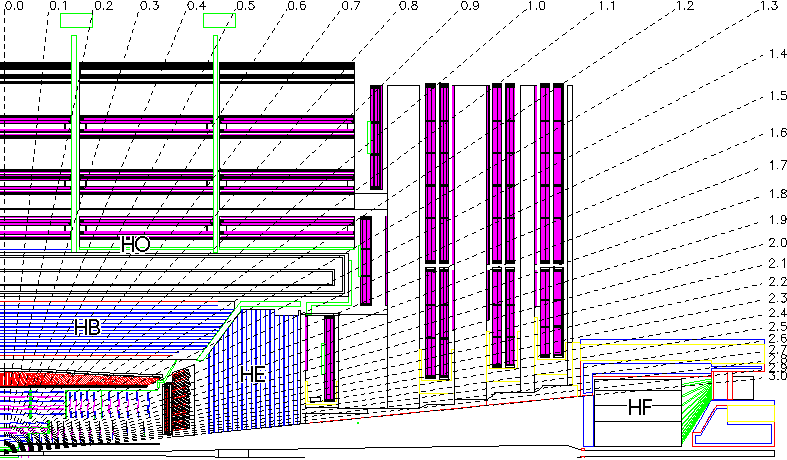
\includegraphics[width=0.95\textwidth]{figures/experiment/CMS_hcal.pdf}
}

The inner hadron calorimeter, consisting of a barrel~(\gls{hb}) and two endcap~(\gls{he}) regions, is located directly after the \gls{ecal} and extends up to the solenoid. The \gls{hb} covers a pseudorapidity range of $|\eta|<1.3$. It consists of brass absorber plates in 14 layers oriented along the z-axis with a thickness of 50.5~mm~(first eight) and 56.5~mm~(last six) respectively. For structural support two additional layers of 40~mm and 50.5~mm thick steel absorber plates are installed at the inner and outer rim respectively. Between the absorbers 72 azimuthal wedges of plastic scintillators in 17 layers with a thickness of 3.7~mm or 9~mm are installed where each covers a segment of $\Delta\eta\times\Delta\phi=0.087\times0.087$. Their emitted light is optically added per tower and guided through \gls{wls} fibers to \glspl{hpd} located at the end of the \gls{hb} structure. The \gls{hb} has a depth of 5.8 interaction lengths at $\eta=0$ which increases with pseudorapidity and amount to 10.4 interaction lengths at $|\eta|=1.3$. 

The same design of alternating brass absorbers~(79~mm thick) with 17 scintillator layers in-between and \gls{wls} fibers for readout is utilized in the \gls{he}. It covers a pseudorapidity range of $1.3<|\eta|<3$ and has a depths of about ten interaction lengths. Its granularity changes from $\Delta\eta\times\Delta\phi=0.087\times0.087$ to $0.17\times0.17$ for $|\eta|>1.6$.

To further contain hadronic showers in the barrel region, an additional calorimeter, the hadron outer calorimeter~(\gls{ho}), is placed directly at the outside of the solenoid utilizing it as an absorber. It consists of one or two layers of scintillators, depending on the pseudorapidity, which match the granularity of the \gls{hb}. This extends the depths of the combined \gls{hb}+\gls{he}+\gls{ho} system to an overall minimum of 11.8 interaction length with the exception of the \gls{hb}-\gls{he} transition region.

An additional calorimeter system, the hadron forward calorimeter~(\gls{hf}), is located 11.2~m away from the \gls{ip} at both sides where it covers a pseudorapidity range of $3<|\eta|<5.2$. A different detector technology was chosen for the \gls{hf} to withstand the expected higher levels of radiation of about $1~\mathrm{MGy/a}$ in the forward region. The calorimeter utilizes quartz fibers to detect Cherenkov light from the electromagnetic component of a shower. The fibers are oriented along the z-axis and placed grooves within steel plates which act as absorbers. The fibers are arrange to achieve a granularity of $\Delta\eta\times\Delta\phi=0.175\times0.175$. Only half of the fibers extend over the complete \gls{hf} depth of 165~cm which corresponds to 10 interaction lengths. The other half starts at a depths of 22~cm instead. Since the electromagnetic showers are typically shorter than hadronic ones the showers can be disentangled from each other by comparing the separated readouts from the long and short fibers. The produced Cherenkov light is detected by \glspl{pmt} located behind a shield of 40~cm steel and polyethylene slabs which protects them from the high radiation. 

The \gls{hf} is of particular importance for this thesis since the signature of t-channel single top quark events feature a characteristic forward jet that is often detected within its acceptance.


%##############################################
\subsection{Muon systems}
%##############################################
\label{sec:experiment-muon-systems}

A major design goal of \gls{cms}, is the precise and robust detection of muons to achieve a good dimuon mass resolution~($1\%$ at $100~\GeV$) and charge determination over a wide muon momentum range of up to 1~\TeV and beyond. Reconstructed muons are key ingredients to detect signatures of various \gls{sm} processes and beyond as for example in the investigation of Higgs bosons decaying to four muons via intermediate Z~bosons. In particular, muons which may originate from decays of single top quarks via W~bosons are analyzed in this thesis.

The muon system is located at the outside of the \gls{cms} detector within the gaps of the iron yoke. It consists of three types of gaseous detectors. An overview is provided in Fig.~\ref{fig:experiment-muons}. \Glspl{dt} are installed in the barrel~($|\eta|<1.2$) where the muon flux is low. In the endcaps~($0.9<|\eta|<2.4$), \glspl{csc} are used which can operate in the higher muon flux environment and in the inhomogeneous magnetic field. In addition, \glspl{rpc} are installed in the barrel and endcaps as a complementary system with a coverage of $|\eta|<1.6$.

\myfigure{\label{fig:experiment-muons}Overview of the \gls{cms} muon system by the end of \gls{lhc} Run~1. The figure is taken from Ref.~\cite{Chatrchyan:2013sba}.}{
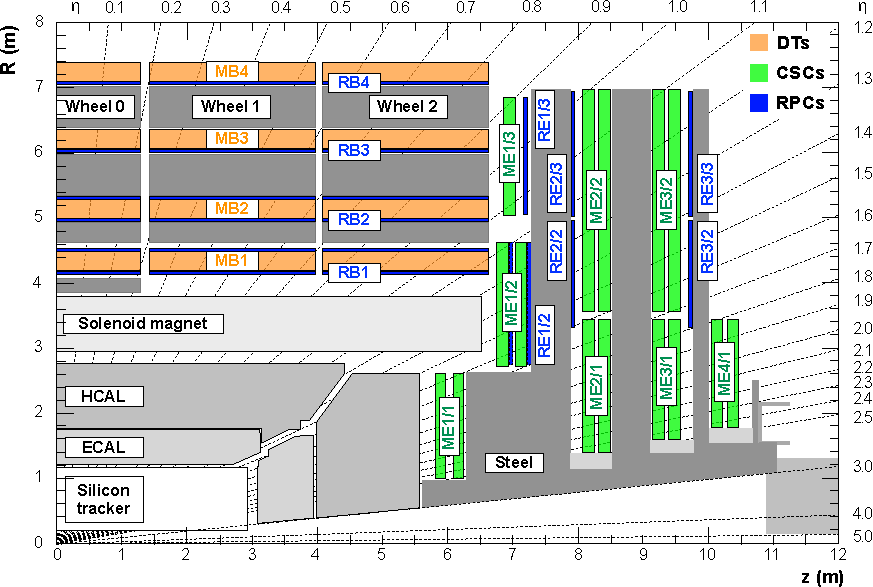
\includegraphics[width=0.85\textwidth]{figures/experiment/CMS_muons.pdf}
}

The \glspl{dt} consist of nearly rectangular cells with a cross section of $42\times 13~\mathrm{mm}^{2}$ in which a $50~\upmu\mathrm{m}$ thick and 2.4~m long gold-plated steel wire is spanned through the center. The cells are filled with a gas mixture of 85\%~Ar and 15\%~$\mathrm{CO}_{2}$ which yields a gain of $10^{5}$ and a drift time of about 380~ns for a maximum drift length of 21~mm. The \glspl{dt} are organized in four layers which form an independent gas-tight super layer unit. A \gls{dt} chamber consists three (or two) super layers where the wires in the first and last layers are oriented along the z-axis and the wires in the middle layer are oriented orthogonal along the $\phi$ direction. There are four layers of \glspl{dt} chambers placed in the barrel region where 60~chambers are installed in each of the inner three layers and 70 in the outer one which amounts to about 172'000 wires in total. 

In the endcaps, trapezoidal-shaped \glspl{csc} are installed in four layers where each layer consists of 18 or 36 chambers which are slightly overlapping to ensure full azimuthal coverage. They are multiwire proportional chambers where each consists of seven radially-orientated cathode strips glued on 12.7~mm-thick panels. Their pitch changes radially from 8.4~mm to 16~mm at the outside. Six azimuthally-orientated wires are placed in the gas gaps between the panels with a width of 9.5~mm. A gas mixture of 40\%~Ar, 50\%~$\mathrm{CO_{2}}$, and 10\%~$\mathrm{CF}_{4}$ is used which yields a gain of about $7\times10^{4}$ at a voltage of $3.6~\mathrm{kV}$. Since the first inner \glspl{csc}~(labeled ME1/1) are located inside the solenoid a slightly different design with tilted wires by $29^{\circ}$ was chosen to compensate for the Lorentz drift in the large magnetic field. The forth \gls{csc} layer labeled ME4/2 (not present in Fig.~\ref{fig:experiment-muons}) has been installed after the \gls{lhc} Run~1 which adds an additional redundancy for muons within $1.2<|\eta|<1.8$~\cite{Wulsin:2015shd}.

The muon system is completed by \glspl{rpc} in the barrel and endcaps. These are gaseous parallel-plate detectors with two gaps of 2~mm width each. They provide a much shorter time resolution than the \glspl{dt} and \glspl{csc} of about 1~ns. Hence they are used to associate a muon signal to the corresponding \gls{lhc} bunch crossing. In the barrel, six layers of \glspl{rpc} are installed with their strips oriented along the z-axis. Their pitch varies per layer such that an azimuthal granularity of $5/16^\circ$ is achieved. In the endcaps, four \gls{rpc} layers are installed with radially oriented strips. The forth layer was added after the \gls{lhc} Run~1~\cite{Tytgat:2012xi}.



%##############################################
\subsection{Data acquisition}
%##############################################


The \gls{cms} \gls{tridas}~\cite{Cittolin:578006,Bawej:2015tmz} deals with the individual readouts of the various subdetector front-end systems. It associates them to an event and finally transmits a file of multiple events to the \gls{cern} computing cluster for storage. A two-staged event triggering system is employed whose aim is to reduce the high data rate and select only events for storage of certain physics interest. The event rate from the bunch crossing frequency of 40~MHz is reduced to about 100~kHz after the first stage, the \gls{l1} trigger, and then to less than 1~kHz after the final \gls{hlt} system.

The data acquisition begins at the subdetector systems where the readout is stored continuously in pipelined buffers at 40~MHz. The \gls{l1} trigger system analyzes only the readouts from the calorimeter and muon systems per bunch crossing to take a decision within a latency of . It consists widely of \glsreset{fpga}\glspl{fpga} which enable a flexible adaptation of the system to potential varying conditions and needs. The regional~(\gls{rct}) and global calorimeter trigger systems~(\gls{gct}) attempt to locate electron, photon, jet, and $\tau$-jet candidates from the \gls{ecal} and \gls{hcal} readouts. Additional information like the missing transverse energy and number of jets are also determined. The global muon trigger system~(\gls{gmt}) attempts to find muon candidates by utilizing local information from the independent \gls{dt}, \gls{csc}, and \gls{rpc} trigger systems. In addition, a muon is considered isolated if the hadronic activity in its vicinity (provided by the \gls{gct}) is below a certain threshold. The final \gls{l1} decision is taken by the \gls{gt} based on the candidates found by the \gls{gct} and \gls{gmt} systems.

After a positive \gls{l1} decision is received the readout fragments with a size of up to 8~kB are transfered via optical links by the \glspl{fed} to readout units~(\glspl{ru}) where multiple fragments are merged. Event builder units~(\glspl{bu}) pick up the fragments via a high speed, Infiniband-based switching network from the \glspl{ru} and assemble the events.

The \gls{hlt} system is part of the standard \gls{cms} software~(\gls{cmssw}) and runs on filter units~(\glspl{fu}) that read the assembled events from the \glspl{bu} via an Ethernet network. Starting from the \gls{l1} candidates, the complete readout of an event is subjected to a sequence of reconstruction and filtering steps to reach a \gls{hlt} decision. One output file is created per \gls{cmssw} process, \gls{hlt} stream, and luminosity section where the latter corresponds to a period of about 23~s. The files are merged in two steps on the \glspl{fu} and \glspl{bu} before they are transfered to the \gls{cern} computing center.
